\chapter{El electrón en la red periódica}

\section{Teoría de Bandas}\label{cap:1}
El problema de la movilidad de los electrones en los sólidos y la existencia de conductores y aislantes seguía siendo un misterio a principios del siglo XX. El modelo de Drude, propuesto en el año 1900, modela los electrones en el sólido como un gas ideal de partículas clásicas, que se mueven aleatoriamente en linea recta e interactúan a través de colisiones con los núcleos inmóviles de los átomos. Dos cantidades físicas son importantes en este modelo: el tiempo entre colisiones $\tau$ y el camino libre medio entre colisiones $l$. El modelo de Drude fue exitoso en explicar el efecto Hall, la conductividad térmica y eléctrica; pero no explica por qué algunos sólidos presentan conductividad eléctrica y otros no \cite{kittel}.

Para entender la conductividad de los distintos materiales, es necesario tomar en consideración la naturaleza cuántica y la estructura interna periódica cristalina del sólido. El descubrimiento de la teoría cuántica y el principio de exclusión de Pauli permitieron que Sommerfield resolviera el problema del calor específico, el cual no había sido resuelto por Drude. El modelo de Somerfield estudia, de forma muy similar a Drude, al gas de electrones, pero tomando en cuenta la estadística de Fermí-Dirac en sus cálculos. Ambos modelos, llamados en conjunto \textit{Modelo de Electrones Libres} permiten tener una idea acertada sobre la capacidad térmica, la conductividad térmica, la conductividad eléctrica, la susceptibilidad magnética y la electrodinámica en los metales, pero no resuelve el problema de la conducción en metales, semimetales, semiconductores y aislantes \cite{ashc}.

La Teoría de Bandas permite explicar la diferencia en la conductividad eléctrica de los conductores, semiconductores y aisladores \cite{valen}. El trabajo de Bloch sobre las funciones ondulatorias de electrones en la red cristalina y los casi simultáneos trabajos de Pierls y Bethe, abrieron el camino de la Teoría de Bandas. La alta conductividad no se relaciona directamente con un alto grado de movilidad de los electrones, pues estos necesitan encontrar estados libres en las bandas de energía; si tales estados no existen, el cristal será un aislante \cite{Kragh}.

En un átomo aislado, los electrones ocupan orbitales bien definidos de energía que están cuantizados. Cuando dos átomos idénticos se acercan para formar una molécula, las funciones de onda de los electrones que ocupan los mismos orbitales en cada uno de los átomos comienzan a interactuar. El principio de exclusión de Pauli, impide que existan dos electrones en el mismo estado cuántico compartiendo un mismo orbital, debido a esto, dichos orbitales experimentan una separación de los estados, separándose las energías y apareciendo dos nuevos estados discretos. En los sólidos, este mismo proceso ocurre en el orden de $10^{23}$ veces, ocasionando que la separación de los estados sea muy pequeña (del orden de $10^{-23}$ eV), esto crea un cuasicontínuo de niveles de energía que se denomina banda. En un cristal de $N$ sitios, si se toma en cuenta que por cada estado cuántico puede existir dos electrones con spin opuesto, se tendrá $2N$ estados permitidos para llenar la banda.

Para un electrón libre, la energía está dada en $k$:

\begin{equation}\label{eq:1.1}
    E_k=\frac{\hbar^2k^2}{2m}\,.
\end{equation}

En ausencia de cualquier interacción entre orbitales, los niveles de energía electrónicos están dados por una parábola en el espacio $k$. Esto se mantiene cierto incluso cuando se incluye un potencial periódico débil, excepto en la zona cercana a los \textit{Planos de Bragg}. En este modelo, llamado del \textit{Electrón casi libre}, la interacción del electrón con el potencial periódico de la red ocasiona una corrección de los niveles de energía del electrón libre cerca de los planos de Bragg. La energía se corrige dibujando otra parábola centrada en $k$, donde $k$ es el vector recíproco del cristal. La curva original se modifica, tal como se muestra en la figura \ref{fig:1.2} a. Esta representación de los niveles de energía se llama \textit{Esquema de zonas extendido} \cite{ashc}. La degeneración de los niveles electrónicos en los planos de Bragg ocasiona que las energías en las cercanías de los planos se separen. La energía del electrón en el modelo del \textit{Electrón casi libre} en dos dimensiones bajo el esquema de perturbación, resulta ser: 

\begin{equation}\label{eq:1.2}
    \mathcal{E}=\mathcal{E}^{K}_{0} \pm |U_K|
\end{equation}

Donde $\mathcal{E}^{K}_0$ es la energía en ausencia del potencial periódico, y $|U_K|$ el módulo de la componente de Fourier del potencial periódico en el el espacio recíproco.

\begin{figure}[H]
    \centering
    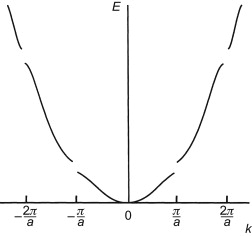
\includegraphics[scale=1]{imagenes/esquema_bandas.jpg}
    \caption{Esquema extendido de bandas, las discontinuidades de la parábola indican bandas prohibidas.}
    \label{fig:1.1}
\end{figure}


 El espacio que se forma debido a la discontinuidad en la curva corresponde a energías prohibidas. Estas regiones se denominan \textit{Bandas prohibidas}  y ningún electrón puede ocupar estos niveles. Como se ha visto, estas  resultan de la interacción de las ondas de electrones de conducción con los núcleos de iones del cristal \cite{kittel}. La forma en que los electrones del solido llenan las bandas permitidas determina si este será un conductor, semiconductor o aislador. Se denomina banda de valencia a la ultima banda totalmente llena del solido,  la banda vacía, inmediatamente por encima de la banda de valencia, se denomina \textit{Banda de Conducción} \cite{valen}.

En la aproximación de \textit{Tight Binding} (sección \ref{cap:5}), el potencial de la red es comparable con la energía del electrón y las funciones de onda de los electrones vecinos se superponen parcialmente. Tomando en consideración solo los primeros vecinos, se obtiene la relación de dispersión:

\begin{equation}\label{eq:1.3}
    \mathcal{E}=\mathcal{E}_0-2A\cos(ak)
\end{equation}

Es evidente, partiendo de esta ecuación, que la energía estará acotada entre dos valores ($\mathcal{E}_0 \pm 2A$) formando las bandas permitidas en el sólido. 

Tanto la aproximación de \textit{Tight Binding}, como la aproximación de electrones casi libres, son útiles dependiendo del sólido a estudiar. El modelo de electrón casi libre es usado frecuentemente en metales, mientras que el modelo de enlace fuerte es bastante usado para semiconductores y aislantes. 
La forma en la que se llenan las bandas determina la conductividad del sólido, el cristal se comporta como un metal si una o más bandas están parcialmente llenas. El cristal es un semiconductor, o un semimetal, si hay bandas están ligeramente llenas o ligeramente vacías \cite{kittel}. A la temperatura de cero absoluto, los electrones llenan las bandas en orden ascendente a partir de su estado mas bajo, hasta una energía dada que se determina de acuerdo al número de estados disponibles, y el numero de electrones del cristal. Este último estado en llenarse es la energía de Fermi del cristal en el cero absoluto \cite{solidos}. En un cristal unidimensional algunas de las bandas permitidas están totalmente llenas, parcialmente llenas o totalmente vacías. Las bandas totalmente llenas o vacías no pueden contribuir a la corriente. En una banda totalmente llena no hay estados disponibles para que los electrones puedan ser excitados gradualmente, por lo que estos electrones se encuentran atrapados en la banda.

En un aislador, el número de electrones del cristal es suficiente para llenar completamente cierto número de bandas, pero la brecha prohibida entre la última banda llena y la primera vacía es tan ancha (alrededor de $15$ eV), que es prácticamente imposible excitar térmicamente un número importante de electrones hacia la banda vacía. Por lo tanto en un aislante solo hay bandas llenas o vacías, y no fluye ninguna corriente de electrones libres.

Si la brecha prohibida en este tipo de sólidos es lo suficientemente pequeña (alrededor de 1 eV), existe una probabilidad estadística apreciable de que los electrones puedan excitarse a estados de la banda vacía, permitiendo un flujo de corriente. A estos materiales se les llama semiconductores. 

\begin{figure}[H]
    \centering
    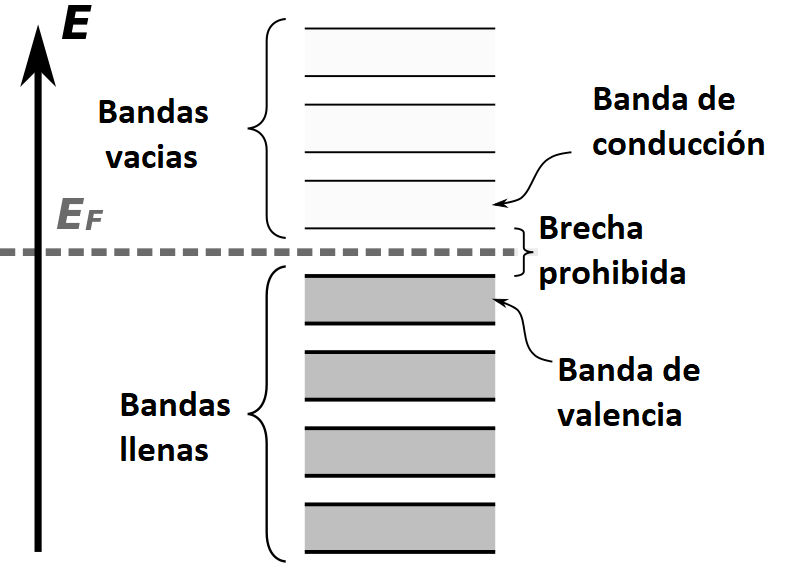
\includegraphics[scale=.5]{imagenes/Semiconductor_band_structure.png}
    \caption{Esquema de bandas para un semiconductor}
    \label{fig:1.2}
\end{figure}

Todo semiconductor tiende a volverse aislador a medida que se enfría el material acercándose al cero absoluto (a excepción de los superconductores) y un aislador puede comportarse como semiconductor si alcanza la temperatura suficiente. Sin embargo, esta situación es muchas veces imposible de obtener en la práctica, ya que el sólido se funde o evapora \cite{solidos}.



%%%%%%%%%%%%%%%%%%%%%%%%%%%%%%%%%%%%%%%%%%%%%%%%%%%%%

\section{Teoría de Floquet}\label{cap:2}

El objetivo de este capítulo consiste en establecer las bases generales del comportamiento de un electrón en una red cristalina unidimensional. Con este fin, se presenta la teoría de Floquet para la solución de ecuaciones diferenciales ordinarias de segundo orden con coeficientes periódicos.

El sobresaliente matemático Achile Marie Gaston Floquet (1847-1920) hizo grandes contribuciones en el campo de las matemáticas y análisis matemático.
En el campo de las ecuaciones diferenciales ordinarias, uno de sus desarrollos mas prominentes es su {\it{Teorema de Floquet}} (1883), que permite obtener una forma canónica para cada matriz fundamental de soluciones a los sistemas de ecuaciones diferenciales lineales periódicas \cite{mananga}. Adicionalmente, la Teoría de Floquet estudia las ecuaciones diferenciales ordinarias periódicas y sus soluciones, así como su estabilidad. 
La Teoría de Floquet es de interés particular cuando se quiere investigar sistemas dinámicos, por ejemplo, a las ecuaciones de Mathieu y las ecuaciones diferenciales de Hill, usadas para aproximar el movimiento lunar.

\subsubsection{Teoría general de Floquet}

El Teorema de Floquet es equivalente al Teorema de Bloch en Física de Materia Condensada \cite{mananga}. Considérese una ecuación diferencial de segundo orden de la forma:

\begin{equation}\label{eq:2.1}
    a_0(x)f''(x)+a_1(x)f'(x)+a_2(x)f(x)=0
\end{equation}

Donde los coeficientes complejos $a_r(x)$ son funciones periódicas y continuas a trozos que comparten exactamente el mismo periodo real: $a>0$ \cite{floquet}:

\begin{equation}\label{eq:2.2}
    a_r(x+a)=a_r(x)\,,\quad{}0\leq{}r\leq{}2\,,
\end{equation}

$a_0(x)$ no se anula en ningún punto de su dominio, evitando así singularidades en la ecuación diferencial. Se sigue que, si $\psi(x)$ es una solución a la ecuación diferencial, entonces $\psi(x+a)$ será también solución, sin decir con esto que $\psi(x)$ es periódica, o que $\psi(x)$ y $\psi(x+a)$ sean la misma función \cite{floquet}. Sin embargo $\psi$ tiene una propiedad, que se expone en el teorema \ref{teo:2.1}.\\

\begin{teo}\label{teo:2.1}

Existe una constante no nula $\rho$ y una solución no trivial $\psi(x)$ de \ref{eq:2.1} tal que se cumple la ecuación \ref{eq:2.3}. \cite{floquet} (apéndice \ref{apendice:A.1}).

\begin{equation}\label{eq:2.3}
    \psi(x+a)=\rho\, \psi(x)
\end{equation}

\end{teo}

\begin{teo}\label{teo:2.2}
Existen soluciones linealmente independientes de \ref{eq:2.1}, $\psi_1(x)$ y $\psi_2(x)$ tales que:

\begin{equation}\label{eq:2.4}
    \psi_1(x)=e^{m_1x}p_1(x)
\end{equation}

\begin{equation}\label{eq:2.5}
    \psi_2(x)=e^{m_2x}p_2(x)
\end{equation}

Donde $m_1$ y $m_2$ son constantes, no necesariamente distintas, y $p_1(x)$ y $p_2(x)$ son periódicas con periodo $a$ \cite{floquet} \ref{apendice:A}. Y en general, existen $k$ soluciones a \ref{eq:2.1} tales que: 

\begin{equation}\label{eq:2.6}
    \psi_k(x)=p_k(x)\,{}e^{m_kx}
\end{equation}

\end{teo}


\subsubsection{Teoría de Floquet en sistemas lineales}

La teoría de Floquet puede extenderse a sistemas lineales, de la siguiente manera:

\begin{equation}\label{eq:2.7}
    f'(x)=C(x)f(x)
\end{equation}

Donde $C(x)$ es una matriz de variable compleja, suave a trozos y de tamaño $n \times n$ tal que: 

\begin{equation}\label{eq:2.8}
    C(x+a)=C(x)
\end{equation}

Donde $a$ es una constante no nula. Denotaremos con minúsculas los vectores de $n$ componentes, y con mayúsculas a las matrices.

\begin{teo}\label{teo:2.3}
Existe una constante no nula $\rho$, y una solución no trivial $\psi(x)$ a \ref{eq:2.7} tal que: 

\begin{equation}\label{eq:2.9}
    \psi(x+a)=\rho \psi(x)
\end{equation}

La prueba a este, es análoga al teorema \ref{teo:2.1} \cite{floquet} \ref{apendice:A}.\\ 
\end{teo}

\begin{teo}\label{teo:2.4}
Existen $n$ soluciones de \ref{eq:2.7} linealmente independientes $\psi_k(x)$ tales que:

\begin{equation}\label{eq:2.10}
    \psi_k(x)=e^{im_kx}p_k(x)
\end{equation}

Sea $\Psi(x)$ la matriz fundamental de \ref{eq:2.7}, entonces se cumple la siguiente igualdad:

\begin{equation}\label{eq:2.11}
    \Psi(x+a)=\Psi(x)B
\end{equation}
\cite{floquet} \ref{apendice:A}
\end{teo}

Estos resultados pueden ser expresados en términos de matrices. Como $B$ es una matriz no singular,existe una matriz $M$ tal que:

\begin{equation}\label{eq:2.12}
    B=e^{Ma}
\end{equation}

Por lo que se define un $P(x)$ análogo a \ref{eq:2.6} y se definen las soluciones al sistema de ecuaciones lineales en la forma \ref{eq:2.13}; donde $P(x)$ es periódico, de periodo $a$ \cite{floquet}:

\begin{equation}\label{eq:2.13}
    \Psi(x)=P(x)e^{Mx}, \     P(x)=P(x+a)
\end{equation}

%%%%%%%%%%%%%%%%%%%%%%%%%%%%%%%%%%%%%%%%%%%%%%%


\section{Teorema de Bloch}\label{cap:3}

En 1928, Felix Bloch, descubrió que el momento cristalino es una cantidad conservada, sin importar lo poderoso que sea el potencial periódico. Este descubrimiento se conoce como el Teorema de Bloch, y establece que un electrón en un potencial periódico tiene autoestados de la siguiente forma \cite{oxford}:

\begin{equation}\label{eq:3.1}
\Psi_{k}(x)=e^{ikx}u_{k}(x)
\end{equation}

Donde $u(k)$ es periódico en la celda unitaria y k (el momento cristalino) puede elegirse dentro de la primera zona de Brillouin \cite{oxford}. Las funciones propias de la ecuación de ondas para un potencial periódico son el producto de una onda plana $e^{ikx}$ por una función $u_k(x)$ que posee la periodicidad de la red cristalina \cite{kittel}.

El teorema de Bloch propone una forma para las funciones de onda asociadas a un electrón en presencia de un potencial perfectamente periódico. Sea una ecuación diferencial que tiene la forma de la siguiente ecuación \cite{solidos}:

\begin{equation}\label{eq:3.2}
    \frac{d^2\Psi(x)}{dx^2}+V(x)\Psi(x)=0
\end{equation}

Donde $V(x)$ es una función periódica con periodo del parámetro de red $a$, que corresponde a la distancia que existe entre los iones del cristal, en este caso unidimensional (ver figura \ref{fig:3.1}).

\begin{figure}[H]
    \centering
    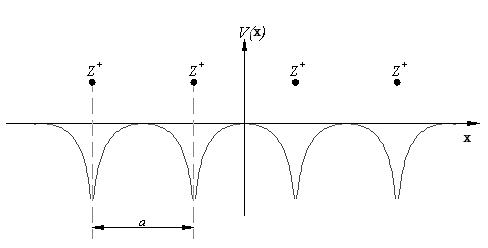
\includegraphics{imagenes/potencial-red.png}
    \caption{Potencial periódico de la red, imagen referencial tomada de http://en.wikipedia.org en.wikipedia}
    \label{fig:3.1}
\end{figure}

Tomando en cuenta el teorema \ref{teo:2.1}, se pueden definir soluciones $\Psi(x)$ para la ecuación \ref{eq:3.2}, que cumplen con las condiciones siguientes:

\begin{equation}\label{eq:3.3}
    \Psi(x+a)=\rho\,\Psi(x),\qquad{} \rho=e^{ika}
\end{equation}

Se sabe por el teorema \ref{teo:2.1} que $\Psi(x)$ puede escribirse como sigue, donde se define un $u_k(x)$ periódico, de periodo $a$:  

\begin{equation}\label{eq:3.4}
    \Psi_k(x)= e^{ikx}u_k(x)
\end{equation}

\begin{equation}\label{eq:3.5}
    u_{k} (x+a) =u(x)_{k}
\end{equation}

La ecuación \ref{eq:3.4} son las llamadas \textit{Funciones de Bloch}. Como se puede notar, se trata de ondas planas, con vector de propagación $k$ y que están moduladas por funciones periódicas $u(x)_k$ (ver figura \ref{fig:3.2}).

\begin{figure}[H]
    \centering
    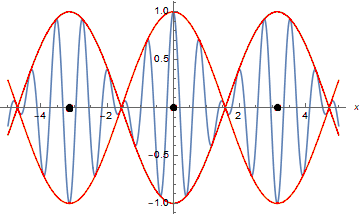
\includegraphics[scale=.7]{imagenes/Bloch_function.png}
    \caption{Funciones de Bloch, dibujo referencial}
    \label{fig:3.2}
\end{figure}

Se concluye entonces que la red tiene el efecto de deslocalizar el paquete de onda del electrón, de tal manera que ya no es posible determinar la posición del electrón en un punto específico del sólido. 
Ahora, se aplican condiciones de frontera periódicas de Born–von Karman sobre $\Psi(x)$ (ecuación \ref{eq:3.6}). Estas son condiciones de frontera que permiten establecer una continuidad en el solido finito. Se supone que la red está compuesta por N sitios, y que el valor de la función en la primera posición es igual a la ultima posición, esto se conoce también como red de anillo \cite{solidos}. Las condiciones Born–von Karman implican que $e^{ikNa}=1$. De esta expresión se obtiene que $k$ tiene valores bien definidos dados por la ecuación \ref{eq:3.7}:

\begin{equation}\label{eq:3.6}
    \Psi_k(x+Na)=e^{ikNa}\Psi_k(x)=\Psi_k(x)
\end{equation}

\begin{equation}\label{eq:3.7}
k_n=\frac{2\pi n}{Na}, \ n={0,1,2,...,N}
\end{equation}

De este resultado se obtiene que el electrón puede tener tantos estados posibles de $k$ como sitios posea la red.

%%%%%%%%%%%%%%%%%%%%%%%%%%%%%%%%%%%%%%%%%%%%%%%%%%%%%

\section{Ecuaciones de Hill}\label{cap:4}

Las ecuaciones de Hill pertenecen a la clase de ecuaciones diferenciales lineales homogéneas de segundo orden con coeficientes reales periódicos. A pesar de que estas ecuaciones fueron investigadas desde mucho antes de la publicación sobre el movimiento lunar de Hill en 1877 \cite{moon}, se les ha dado ese nombre por sus importantes contribuciones a la teoría. Las ecuaciones de Hill tienen muchas aplicaciones en problemas de ingeniería y física, en especial para mecánica, astronomía, teoría de circuitos eléctricos, y la conductividad en metales. 
Un resultado importante de la teoría de Hill es que esta revela la ocurrencia de un fenómeno sorprendente: si una fuerza que varía periódicamente en el tiempo actúa sobre una masa, de tal manera que la fuerza tiende a mover la masa alrededor de una posición de equilibrio, uno puede esperar que la masa se mantenga confinada a una vecindad de la posición de equilibrio. En particular, entre mayor sea la fuerza uno esperaría que esta fuese mas eficiente en este propósito, sin embargo este no es el caso. Un incremento en la fuerza puede causar que la partícula oscile con mayor amplitud cada vez. La teoría de intervalos de estabilidad en las ecuaciones de Hill provee una descripción precisa de este fenómeno.
La ecuación diferencial de Hill tiene la forma general: 

\begin{equation}\label{eq:4.1}
    \frac{\partial^2}{\partial t^2}y+f(t)y=0
\end{equation}

Donde $f(t)$ es una función periódica de periodo $a$, debido a esto, se puede escribir la ecuación en series de Fourier como sigue: 

\begin{equation}\label{eq:4.2}
   \frac{\partial^2}{\partial t^2}y+\left(\theta_0+2\sum^{\infty}_{n=1}\theta_n\cos(2nt)+2\sum^{\infty}_{n=1}\phi_n\sin(2nt)\right)y=0
\end{equation}

Un caso especial para las ecuaciones de Hill son las ecuaciones de Mathieu. En este caso $f(t)$ es una función par y $n=1$.

Émile Léonard Mathieu (1835-1890) fue un matemático francés, cuyas contribuciones más importantes están en la teoría de grupos y la física matemática. Su nombre aparece en las \textit{Ecuaciones de Mathieu}, \textit{Grupos de Mathieu} y la \textit{Transformación de Mathieu}. Su descubrimiento sobre las \textit{Ecuaciones de Mathieu} se produjo mientras estudiaba las vibraciones de la membrana elíptica. La expresión general de la ecuación de Mathieu tiene la siguiente forma:

\begin{equation}\label{eq:4.3}
    \frac{\partial^2u}{\partial Z^2}+\left(\theta_0+2\theta_1\cos(2Z)\right)u=0
\end{equation}

Muchas propiedades de las \textit{Ecuaciones de Mathieu} se pueden deducir a partir de la \textit{Teoría de Floquet}. Aparecen en un gran número de contextos en ingeniería, física, y matemática aplicada. Tiene aplicaciones en el estudio de ecuaciones con geometría elíptica, y también se aplican a problemas dinámicos con fuerzas que son periódicas en el espacio o en el tiempo.
Las \textit{Funciones de Mathieu} juegan un papel importante en sistemas mecánico-cuánticos, en especial aquellos que incluyen potenciales periódicos, por ejemplo, el péndulo cuántico y las redes cristalinas. Se verá, mas adelante, que la ecuación de Schrödinger, que describe al electrón en la red de Enlace Fuerte y en presencia del potencial rápidamente oscilante, es una ecuación diferencial de Hill o de Mathieu. A continuación se describirá un método analítico para hallar las soluciones a esta ecuación diferencial.
En 1868, Mathieu halló que la \textit{serie periódica doble} es solución a la ecuación diferencial de Mathieu.

\begin{teo}{\textbf{Teorema de Floquet}}\label{teo:4.1}:
Debe ser posible encontrar dos soluciones diferentes de la forma $x=e^{i\lambda z}$ multiplicada por una serie de Laurent en $x^2$. Una serie de Laurent en $x^2$ es una serie de potencias enteras positivas y negativas de x, esto es, una
serie de Fourier en $2z$. Esta serie es periódica en $z$,con periodo $\pi$, y puede representar la función alrededor de los puntos singulares $x = 0$ y $x = \infty$. Escogemos entonces a la ecuación \ref{eq:4.4} como una solución \cite{Philip}:

\begin{equation}\label{eq:4.4}
    u=e^{i\lambda z}\sum^{\infty}_{n=-\infty} b_n e^{2inz}
\end{equation}

\end{teo}

La ecuación \ref{eq:4.4} es una solución a la ecuación de Mathieu, donde $\lambda$ es una  constante, $e^{i\lambda Z}$ representa a la oscilación efectiva, y la suma representa a los armónicos de la oscilación forzada \cite{Phelps}.
Es importante resaltar que la suma es una serie que converge rápidamente ($b_{n+1}$), esto será de utilidad más adelante.
Siguiendo el procedimiento en la sección \ref{cap:5}, se obtiene la condición que debe cumplirse para que la solución $u$ sea distinta a la solución trivial ($u=0$):

\begin{equation}\label{eq:4.5}
\Delta(0)\sin^2(\frac{\pi}{2}\theta_o^{1/2})=\sin^2(\frac{\pi}{2}\lambda)
\end{equation}

Donde $\lambda$ debe ser real para que las soluciones sean estables, y $\Delta(0)$ es el determinante de una matriz infinita . Dicha matriz representa el sistema de ecuaciones infinito que surge de aplicar la solución \ref{eq:4.4} sobre la ecuación diferencial de Mathieu. Este determinante se puede truncar hasta cierto orden, ya que $b_n$ decrece muy rápidamente, se supone además que $\theta_o \ll 1$. Si se desea aproximar hasta orden de $n=1$ se tendrá lo siguiente:

\begin{equation}\label{eq:4.6}
\begin{aligned}
& \Delta_{(0)}^1=
\begin{vmatrix}
 1 & \frac{\theta_1}{-4} & 0 \\ 
\frac{\theta_1}{\theta_o} & 1 & \frac{\theta_1}{\theta_o}  \\
 0 & \frac{\theta_1}{-4} & 1 &  
\end{vmatrix}
= 1+\frac{\theta_1^2}{2\theta_o}
\end{aligned}
\end{equation}

\begin{equation}\label{eq:4.7}
(1+\frac{\theta_1^2}{2\theta_o})\frac{\pi^2}{4}\theta_o=\sin^2(\frac{\pi}{2}\lambda) = Q, \ \  0 \leq Q \leq 1
\end{equation}

Mas adelante se encuentra que para el electrón en la red de \textit{Enlace Fuerte}, forzado por campos eléctricos rápidamente oscilantes, la ecuación de Schrödinger del electrón puede aproximarse a una ecuación diferencial de Hill. Se encuentra, que la condición de no trivialidad para las soluciones de la ecuación diferencial, determina las autoenergías posibles para el electrón en el sistema (capítulo \ref{cap:10}). 

\subsection{Solución de las ecuaciones de Mathieu}

En esta sección se mostrará el procedimiento detallado para la obtención de las condiciones para que la solución a la ecuación de Mathieu sea la no trivial. Como ya se dijo, la forma general de la ecuación de Mathieu tiene la forma:

\begin{equation}\label{eq:E.1}
    \frac{\partial^2u}{\partial Z^2}+\left(\theta_0+2\theta_1\cos(2Z)\right)u=0
\end{equation}

Con solución 

\begin{equation}\label{eq:E.2}
    u=e^{i\lambda z}\sum^{\infty}_{n=-\infty} b_n e^{2inz}
\end{equation}

Se escribe  $\cos(2Z)$ en su forma exponencial y se substituye la solución \ref{eq:E.2} en la \textit{Ecuación Diferencial de Mathieu} \ref{eq:E.1} 


\begin{equation}\label{eq:E.3}
    \cos(2Z)=\frac{e^{2iZ}+e^{-2iZ}}{2}
\end{equation}

\begin{equation}\label{eq:E.4}
    \sum^{\infty}_{n=-\infty} b_n\left(-(\lambda+2n)^2+\theta_0\right)e^{i\left(\lambda+2n\right) Z}+\theta_1\left( b_ne^{i\left(\lambda+2n+2\right)Z}+b_ne^{i\left(\lambda+2n-2\right)Z}\right)=0
\end{equation}

Se hacen las substituciones $m=n+1$ y $l=n-1$ sobre \ref{eq:E.4}:

\begin{equation}\label{eq:E.5}
    \sum^{\infty}_{n=-\infty} b_n\left(\theta_0-\left(\lambda+2n\right)^2\right)e^{i\left(\lambda+2n\right) Z}+\theta_1\left( \sum^{\infty}_{m=-\infty}b_{m-1}e^{i\left(\lambda+2m\right)Z}+\sum^{\infty}_{l=-\infty}b_{l+1}e^{i\left(\lambda+2l\right)Z}\right)=0
\end{equation}

No hay pérdida de la generalidad si se devuelve el cambio haciendo $n=m=l$ en la sumas; obteniendo:

\begin{equation}\label{eq:E.6}
    \sum^{\infty}_{n=-\infty} b_n\left(-(\lambda+2n)^2+\theta_0\right)e^{i(\lambda+2n) Z}+\theta_1( b_{n-1}e^{i(\lambda+2n)Z}+b_{n+1}e^{i(\lambda+2n)Z})=0
\end{equation}

El factor $e^{i(\lambda+2n)Z}$ nunca será cero, se puede dividir la ecuación por este factor y se obtiene un sistema de ecuaciones lineales para los $b_n$ de la solución de la ecuación de Mathieu; Es menester obtener los valores de estos $b_n$.

\begin{equation}\label{eq:E.7}
    \sum^{\infty}_{n=-\infty} b_n\left(-(\lambda+2n)^2+\theta_0\right) +\theta_1( b_{n-1}+b_{n+1})=0
\end{equation}

Se observa que cuando $n \rightarrow \infty$ la suma tiende a infinito, este es un sistema inestable. Esta situación es análoga a tener un polo de segundo orden \cite{Phelps} en las ecuaciones, para evitar este problema, se divide \ref{eq:E.7} por $\theta_0-4n^2$

\begin{equation}\label{eq:E.8}
    \sum^{\infty}_{n=-\infty} \frac{b_n\left(-(\lambda+2n)^2+\theta_0\right)}{\theta_0-4n^2}+\frac{\theta_1b_{n-1}}{\theta_0-4n^2}+\frac{\theta_1b_{n+1}}{\theta_0-4n^2}=0
\end{equation}

Como $n$ toma valores discretos de $-\infty$ a $\infty$, se tiene el problema de resolver un sistema de ecuaciones homogéneo de dimensión infinita. Se puede escribir el sistema de ecuaciones como una matriz cuadrada infinita de la forma siguiente:

\large
\begin{equation}\label{eq:E.9}
A=
\begin{pmatrix}
\ddots &  \vdots & \vdots & \vdots &\iddots \\
\dots &  \frac{\theta_1}{\theta_o-16} & 0 & 0 & \dots \\[0.3cm]
\dots  & \frac{\theta_o-(\lambda-2)^2}{\theta_o-4} & \frac{\theta_1}{\theta_o-4} & 0 & \dots\\[0.3cm] 
\dots & \frac{\theta_1}{\theta_o} & \frac{\theta_o-\lambda^2}{\theta_o} & \frac{\theta_1}{\theta_o} & \dots \\[0.3cm]
\ldots & 0 & \frac{\theta_1}{\theta_o-4} & \frac{\theta_o-(\lambda+2)^2}{\theta_o-4} & \dots\\[0.3cm]
\ldots & 0 & 0 & \frac{\theta_1}{\theta_o-16} & \dots \\
\iddots & \vdots & \vdots  & \vdots &\ddots \\
\end{pmatrix}
=\begin{pmatrix}
\vdots\\
0\\[0.3cm]
0\\[0.3cm]
0\\[0.3cm]
0\\[0.3cm]
0\\
\vdots
\end{pmatrix}
\end{equation}
\normalsize

Si el determinante de este sistema es distinto de cero ($\det(A)=\Delta(\lambda)\neq 0$), las ecuaciones son linealmente independientes y se puede reducir el sistema a una matriz diagonal; por ende la solución será la trivial y todos los $b_n$ tendrán solución $b_n$=$0$ $\forall$ $n$. Se busca una solución no trivial al sistema, por lo que se supone que el determinante de la matriz es igual a cero.

\large
\begin{equation}\label{eq:E.10}
\Delta(\lambda)=
\begin{vmatrix}
\ddots  & \vdots & \vdots & \vdots & \iddots \\
\dots &  \frac{\theta_1}{\theta_o-16} & 0 & 0 & \dots \\[0.3cm]
\dots & \frac{\theta_o-(\lambda-2)^2}{\theta_o-4} & \frac{\theta_1}{\theta_o-4} & 0 & \dots\\[0.3cm] 
\dots & \frac{\theta_1}{\theta_o} & \frac{\theta_o-\lambda^2}{\theta_o} & \frac{\theta_1}{\theta_o} & \dots \\[0.3cm]
\ldots & 0 & \frac{\theta_1}{\theta_o-4} & \frac{\theta_o-(\lambda+2)^2}{\theta_o-4}  &  \dots\\[0.3cm] 
\ldots & 0 & 0 & \frac{\theta_1}{\theta_o-16} &  \dots \\
\iddots &  \vdots & \vdots & \vdots  &\ddots \\
\end{vmatrix}=0
\end{equation}
\normalsize

Se define una matriz diagonal $D$ y una matriz $C$ cuyo valor es:

\begin{equation}\label{eq:E.12}
    C=A*D
\end{equation}:

\large
\begin{equation}\label{eq:E.11}
D= \begin{pmatrix}
\ddots & \vdots & \vdots & \vdots & \iddots \\
\dots & \frac{\theta_o-4}{\theta_o-(\lambda-2)^2} &0 & 0 & \dots \\[0.3cm] 
\dots & 0 & \frac{\theta_o}{\theta_o-\lambda^2} & 0 & \dots \\[0.3cm]
 \dots & 0 & 0 & \frac{\theta_o-4}{\theta_o-(\lambda+2)^2} & \dots \\[0.3cm]
 \iddots & \vdots & \vdots & \vdots& \ddots
\end{pmatrix}
\end{equation}
\normalsize

Al multiplicar $A$ por $D$ explícitamente se obtiene:

\large
\begin{equation}\label{eq:E.13}
C= 
\begin{pmatrix}
\ddots & \vdots & \vdots & \vdots & \iddots \\
\dots & 1 & \frac{\theta_1}{\theta_o-(\lambda-2)^2} & 0 & \dots \\ 
\dots  & \frac{\theta_1}{\theta_o-\lambda^2} & 1 & \frac{\theta_1}{\theta_o-\lambda^2} &\dots\\
 \dots  & 0 & \frac{\theta_1}{\theta_o- (2+\lambda)^2} & 1 & \dots\\ 
 \iddots & \vdots & \vdots & \vdots & \ddots
\end{pmatrix}
\end{equation}
\normalsize 

\begin{teo}
 Sean A y B dos matrices $n\times n$ arbitrarias, entonces $det(A*B)=det(A)*det(B)$\cite{jacob}
\end{teo}


\begin{equation}\label{eq:E.14}
C=AD \Rightarrow \det C= \det A \det D
\end{equation}

Sea $\det(C)=\Delta(\lambda){i}$ entonces, la matriz $\Delta(\lambda){i}$ está definida como:

\begin{equation}\label{eq:E.15}
\Delta(\lambda){i}=\det D *\Delta(\lambda)
\end{equation}

Es inmediato que el determínate de una matriz diagonal es igual a la multiplicación de los elementos de su diagonal, se tiene:

\begin{equation}\label{eq:E.16}
   \det D= \prod_{n=-\infty}^{n=\infty} \frac{\theta_o-4n^2}{\theta_o-(2n+\lambda)^2}
\end{equation}

Sultituyendo \ref{eq:E.16} en \ref{eq:E.15}

\begin{equation}\label{eq:E.17}
\Delta(\lambda)_{i} = \prod_{n=-\infty}^{n=\infty} \frac{\theta_o-4n^2}{\theta_o-(2n+\lambda)^2} \Delta(\lambda)
\end{equation}

Se despeja $\Delta(\lambda)$ para obtener:

\begin{equation}\label{eq:E.18}
\begin{aligned}
\Delta(\lambda) & =\Delta(\lambda)_{i} \prod_{n=-\infty}^{n=\infty} \frac{\theta_o-(2n+\lambda)^2}{\theta_o-4n^2} \\
& = \Delta(\lambda)_{i} \prod_{n=-\infty}^{n=\infty} \frac{[\theta_o^{1/2}-(2n+\lambda)][\theta_o^{1/2}+(2n+\lambda)]}{\theta_o-4n^2} 
\end{aligned}
\end{equation}

Se sigue el procedimiento algebraico que se muestra en el apéndice \ref{apendice:E} y se obtiene:

\begin{equation}\label{eq:E.20}
\begin{aligned}
\Delta(\lambda) & =\Delta(\lambda)_{i} \frac{\theta_o-\lambda^2}{\theta_o}\prod_{n=1}^{n=\infty} [1-(\frac{\theta_o^{1/2}-\lambda}{2n})^2][1-(\frac{\theta_o^{1/2}+\lambda}{2n})^2]\frac{1}{(1-(\frac{\theta_o^{1/2}}{2n})^2)^2}
\end{aligned}
\end{equation}

De la teoría de variable compleja, se sabe que $\frac{\sin(z)}{z}$  satisface la siguiente igualdad \cite{Philip}

\large
\begin{equation}\label{eq:E.21}
\frac{\sin(z)}{z} = \prod_{n=1}^{\infty} 1-(\frac{z}{n \pi})^2
\end{equation}
\normalsize

Y haciendo los cambios:

\Large
\begin{equation}\label{eq:E.22}
\begin{cases}
\frac{z_1}{n\pi}=\frac{\theta_o^{1/2}-\lambda}{2n}\\
\frac{z_2}{n\pi}=\frac{\theta_o^{1/2}+\lambda}{2n}\\
\frac{z_3}{n\pi}= \frac{\theta_o^{1/2}}{2n}
\end{cases}
\end{equation}
\normalsize

 Queda que el determinante que se busca tiene la forma:

 \begin{equation}\label{eq:E.23}
 \Delta(\lambda)= \Delta(\lambda)_{i}\frac{ \theta_o-\lambda^2}{\theta_o}\frac{\frac{\sin(\frac{\pi}{2}(\theta_o^{1/2}-\lambda))}{\frac{\pi}{2}( \theta_o^{1/2}-\lambda)}\frac{\sin(\frac{\pi}{2}( \theta_o^{1/2}+\lambda))}{\frac{\pi}{2}( \theta_o^{1/2}+\lambda)}}{\frac{\sin^2(\frac{\pi}{2}\theta_o^{1/2})}{(\frac{\pi}{2}\theta_o^{1/2})^2}}
 \end{equation}

 
Haciendo simplificaciones se obtiene el resultado:
 
%%%%%%%%%%%%%%%%%%%%%%%%%%%%%%%%%%%

 \begin{equation}\label{eq:2.20}
 \Delta(\lambda)= -\Delta(\lambda)_{i}\frac{\sin(\frac{\pi}{2}(\lambda-\theta_o^{1/2}))\sin(\frac{\pi}{2}( \lambda+\theta_o^{1/2}))}{\sin^2(\frac{\pi}{2}\theta_o^{1/2})}
\end{equation}
\normalsize

Con $\Delta(\lambda)_i$ definida como: 

\begin{equation}\label{eq:2.21}
\Delta(\lambda)_{i} = \prod_{n=-\infty}^{n=\infty} \frac{\theta_o-4n^2}{\theta_o-(2n+\lambda)^2} \Delta(\lambda)
\end{equation}

Siguiendo la teoría de variable compleja, encontramos la siguiente definición:

\begin{defi}{\textbf{Función Meromórfica}}\label{def:1}
Se dice que una función $f(z)$ es Meromórfica en una región, cuando todas sus singularidades $a_n$ en esa región son polos.
Una función que es Meromórfica puede expandirse en serie de fracciones parciales tal como cualquier otra función racional pudiera hacerlo. Pero lo haremos de manera que cada sumando contenga un solo polo\cite{Philip}.

\begin{equation}\label{eq:2.22}
    f(z)=\sum \frac{c_n}{z-a_n}
\end{equation}
\end{defi}

Si se toma un círculo de radio R finito alrededor del origen, dentro del cual se encuentran $p$ polos, y $f(z)$ no tiene polos en la frontera del círculo ni el origen, se puede definir una función analítica cuya expresión es:

\begin{equation}\label{eq:2.23}
    g_p(z)=f(z)-\sum^{p}_1 \frac{c_n}{z-a_n}
\end{equation}

Si se hace crecer el círculo cada vez más, haciendo $R \rightarrow \infty$ la región en la cual $g_p(z)$ es analítica crece. Si existe $M_p$ tal que $\abs{f(z)}\leq M_p$ en la frontera del círculo (recordemos que ningún polo se encuentra en la frontera), y que $M_p$ esta acotada para todo radio. Decimos que $g_p(z)$ está acotada por $M_p$.

\begin{teo}\label{Teo:6}
 Una función que es analítica para todos los valores finitos de z y está acotada en todas partes es una constante.\cite{Philip}
\end{teo}

\begin{equation}\label{eq:2.24}
  \abs{g_p(z)} \leq M_p  
\end{equation}


Se encuentra que $g_p(z)=G$, con G constante y que se cumple la siguiente relación:

\begin{equation}\label{eq:2.25}
    f(z)=G+\sum^{\infty}_1 \frac{c_n}{z-a_n}
\end{equation}

Tomando en cuenta el teorema \ref{Teo:6} y la definición \ref{def:1}, se nota que el determinante $\Delta(\lambda)_i$ tendrá infinitas singularidades que son todas polos, que se alejan cada vez mas del origen. Además, es una función analítica, tal como se ha descrito, por lo que se puede encontrar una constante $G$ tal que:
 
 \begin{equation}\label{eq:E.25}
 \begin{aligned}
 G=&\Delta(\lambda)_{i}-\sum^{\infty}_{-\infty} \frac{c_n}{\theta_o-(2n+\lambda)^2}\\
  &=\Delta(\lambda)_{i}-\sum^{\infty}_{-\infty} \frac{c_n}{\theta_o-(2n+\lambda)^2}\\
  &=\Delta(\lambda)_{i}-\sum^{\infty}_{-\infty} \frac{c_n}{\theta_o^{1/2}+2n+\lambda}+\frac{d_n}{\theta_o^{1/2}-2n-\lambda}
 \end{aligned}
 \end{equation}
 


Se puede calcular gracias a teoría de variable compleja que (ver apéndice \ref{apendice:E}):


\begin{equation}\label{eq:E.27}
    \cot(z)=\sum^{\infty}_{-\infty}\frac{1}{(z+\pi n)}
\end{equation}

haciendo la siguientes sustituciones en \ref{eq:E.27},queda lo siguiente::

\begin{equation}\label{eq:E.28}
\begin{aligned}
\begin{cases}
&z_1=\pi \frac{\theta_o^{1/2}+\lambda}{2}\\
&z_2=\pi \frac{\theta_o^{1/2}-\lambda}{2}
\end{cases}
\end{aligned}
\end{equation}

 \begin{equation}\label{eq:E.29}
     G=\Delta(\lambda)_{i}-K\left[\cot(\frac{\pi}{2}(\lambda+\theta_o^{1/2}))-\cot(\frac{\pi}{2}(\lambda-\theta_o^{1/2}))\right]
 \end{equation}

\begin{equation}\label{eq:E.30}
     \Delta(\lambda)_{i}=G+K[\cot(\frac{\pi}{2}(\lambda+\theta_o^{1/2}))-\cot(\frac{\pi}{2}(\lambda-\theta_o^{1/2}))]
 \end{equation}
 
 Cuando $\lambda$ tiende a infinito el determinante $\Delta(\lambda)_{i}$ tiende a 1.
 
 \large
\begin{equation}\label{eq:E.31}
\lim_{\lambda\rightarrow \infty}\Delta(\lambda){i}=\lim_{\lambda\rightarrow\infty} 
\begin{pmatrix}
\ddots & \vdots & \vdots & \vdots & \iddots \\
\dots & 1 & \frac{\theta_1}{\theta_o-(\lambda-2)^2} & 0 & \dots \\ 
\dots  & \frac{\theta_1}{\theta_o-\lambda^2} & 1 & \frac{\theta_1}{\theta_o-\lambda^2} &\dots\\
 \dots  & 0 & \frac{\theta_1}{\theta_o- (2+\lambda)^2} & 1 & \dots\\ 
 \iddots & \vdots & \vdots & \vdots & \ddots
\end{pmatrix}=1
\end{equation}
\normalsize
 
 \begin{equation}\label{eq:2.27}
     \Delta(\lambda)_{i}=1+K[\cot(\frac{\pi}{2}(\lambda+\theta_o^{1/2}))-\cot(\frac{\pi}{2}(\lambda-\theta_o^{1/2}))]
 \end{equation}
  
 Se substituye \ref{eq:2.27} en \ref{eq:2.20}:
 
 \begin{equation}\label{eq:E.33}
    \Delta(\lambda)= -\frac{\sin(\frac{\pi}{2}(\lambda-\theta_o^{1/2}))\sin(\frac{\pi}{2}(\lambda+ \theta_o^{1/2}))}{\sin^2(\frac{\pi}{2}\theta_o^{1/2})}\times\left[1+K\left[\cot(\frac{\pi}{2}(\lambda+\theta_o^{1/2}))-\cot(\frac{\pi}{2}(\lambda-\theta_o^{1/2}))\right]\right]
\end{equation}

Haciendo simplificaciones trigonométricas se llega a:

\begin{equation}\label{eq:E.35}
    \Delta(\lambda)= -\frac{\sin(\frac{\pi}{2}(\lambda-\theta_o^{1/2}))\sin(\frac{\pi}{2}(\lambda+ \theta_o^{1/2}))}{\sin^2(\frac{\pi}{2}\theta_o^{1/2})}+2K\cot(\frac{\pi}{2}\theta_o^{1/2})
\end{equation}

Haciendo $\lambda=0$ se halla el valor de $K$:

\begin{equation}\label{eq:E.36}
    K= \frac{\Delta(0)+1}{2\cot(\frac{\pi}{2}\theta_o^{1/2})}
\end{equation}

Se substituye $K$ en \ref{eq:E.35}:

\begin{equation}\label{eq:E.37}
    \Delta(\lambda)= -\frac{\sin(\frac{\pi}{2}(\lambda-\theta_o^{1/2}))\sin(\frac{\pi}{2}(\lambda+ \theta_o^{1/2}))}{\sin^2(\frac{\pi}{2}\theta_o^{1/2})}+\Delta(0)+1
\end{equation}

Expandiendo los senos en el numerador y usando identidades trigonométricas se obtiene:


\begin{equation}\label{eq:E.38}
\Delta(\lambda)=\Delta(0)-\frac{\sin^2(\frac{\pi}{2}\lambda)}{\sin^2(\frac{\pi}{2}\theta_o^{1/2})}
\end{equation}

Como $\Delta(\lambda)=0$ se hallan las raíces del determinante.

\begin{equation}\label{eq:E.39}
\Delta(0)\sin^2(\frac{\pi}{2}\theta_o^{1/2})=\sin^2(\frac{\pi}{2}\lambda)
\end{equation}

Se puede truncar el determinante hasta cierto orden, $b_n$ decrece muy rápidamente y el elemento central corresponde a $n=0$, se supone además que $\theta_o \ll 1$ 

\begin{equation}\label{eq:E.40}
\begin{aligned}
& \Delta(0)^0=1 \\
& \Delta(0)^1=
\begin{vmatrix}
 1 & \frac{\theta_1}{-4} & 0 \\ 
\frac{\theta_1}{\theta_0} & 1 & \frac{\theta_1}{\theta_0}  \\
 0 & \frac{\theta_1}{-4} & 1 &  
\end{vmatrix}
= 1+\frac{\theta_1^2}{2\theta_o}
\end{aligned}
\end{equation}

\begin{equation}\label{eq:E.41}
\sin^2(\frac{\pi}{2}\theta_o^{1/2}) \approx \frac{\pi^2}{4}\theta_o
\end{equation}

\begin{equation}\label{eq:E.42}
(1+\frac{\theta_1^2}{2\theta_o})\frac{\pi^2}{4}\theta_o=\sin^2(\frac{\pi}{2}\lambda) = Q
\end{equation}

$\lambda$ es real, por lo que:

\begin{equation}\label{eq:E.43}
0 \leq Q \leq 1
\end{equation}

%%%%%%%%%%%%%%%%%%%%%%%%%%%%%%%%%%%%%%%%%%%%%%%%%%%


\subsection{Caso especial}

Si se supone el caso especial de la ecuación de Hill de la forma:

\begin{equation}
    \frac{\partial u}{\partial Z}+\left(\theta_0+2\theta_1\cos(aZ)+2\theta_2\cos(2aZ)\right)u=0
\end{equation}

Con solución

\begin{equation}
    u=\sum^{\infty}_{n=-\infty} b_n e^{ia(n+\lambda)z}
\end{equation}

Un procedimiento análogo al que se ha realizado en este apéndice deja el resultado:

\begin{equation}
\Delta(0)\sin^2(\frac{\pi}{a}\theta_o^{1/2})=\sin^2(\pi\lambda)
\end{equation}

Con $\Delta_{(0)}$ resultante a primer orden:

\begin{equation}
\begin{aligned}
& \Delta(0)^0=1 \\
& \Delta(0)^1=
\begin{vmatrix}
 1 & \frac{\theta_1}{\theta_0-a^2} & \frac{\theta_2}{\theta_0-a^2} \\ 
 \frac{\theta_1}{\theta_0} & 1 & \frac{\theta_1}{\theta_0}  \\
 \frac{\theta_2}{\theta_0-a^2} & \frac{\theta_1}{\theta_0-a^2} & 1 &  
\end{vmatrix}
= 1+\frac{2\theta_1\theta_2^2-\theta_0\theta_2^2-\theta_1^2(\theta_0-a^2)}{\theta_0(\theta_0-a^2)^2}
\end{aligned}
\end{equation}


%%%%%%%%%%%%%%%%%%%%%%%%%%%%%%%%%%%%%%

\section{Tight Binding}\label{cap:5}
La aproximación de \textit{Tight Binding} ofrece un modelo que permite estudiar la dinámica del electrón en la red, frecuentemente para semiconductores y aisladores. El Hamiltoniano del electrón en esta aproximación, tiene la forma de una ecuación de Hill. El caso mas sencillo donde se puede aplicar la teoría de \textit{Tight Binding} para un electrón en presencia de una perturbación, es la perturbación lineal independiente del tiempo, cuyo resultado son las oscilaciones de Bloch. Conociendo el resultado de esta perturbación sencilla, se puede tener una idea de como aplicar el \textit{Tight Binding} para obtener la dinámica de sistemas de mayor complejidad; por ejemplo, la perturbación inhomogénea rápidamente oscilante. 

En el modelo de \textit{Tight Binding} el sólido se modela como una colección de átomos neutros interactuando débilmente. Se supone que los orbitales atómicos están lo suficientemente cerca para que sus funciones de onda puedan interactuar, por lo que se requerirá una corrección al modelo de átomos aislados, pero no están tan cerca para ignorar por completo su individualidad . De tal manera que es necesario hacer correcciones en el Hamiltoniano que describe la dinámica del electrón, esta descripción es especialmente útil para describir las bandas $d$ de los metales de transición o la estructura electrónica de los aisladores \cite{ashc}. A continuación se desarrolla un modelo que describa la energía de un electrón en una red homonuclear, de tamaño N y  unidimensional (ver figura \ref{fig:5.1}).

\begin{figure}[H]
    \centering
    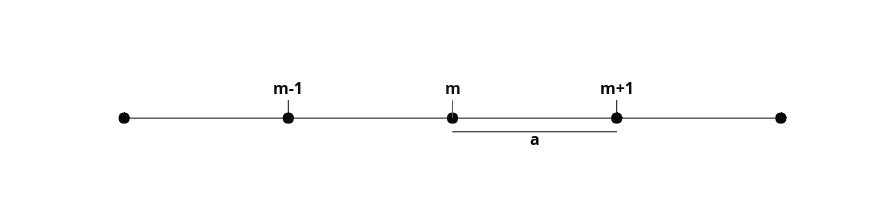
\includegraphics[scale=0.6]{imagenes/red.png}
    \caption{Red infinita homonuclear en una dimensión}
    \label{fig:5.1}
\end{figure}

La primera hipótesis para la construcción del modelo es que en cada sitio $n$, hay un solo orbital $\ket{n}$ que es ortogonal a todos los demás orbitales en los otros sitios de la red \cite{oxford}:

\begin{equation}\label{eq:5.1}
    \braket{n}{m}=\delta_{n,m}\,,
\end{equation}

Se supone adicionalmente que los estados constituyen conjunto completo, tal como se muestra a continuación:

\begin{equation}\label{eq:5.2}
    \sum_n \ket{n}\bra{n}=\mathbf{1}
\end{equation}

La última suposición acerca de la red, es que esta posee $N$ sitios y con condiciones de borde periódicas de Born–von Karman ($\ket{0}=\ket{N}$). Al estar los iones tan cerca unos de otros, la función de onda de cada orbital se superpone con las demás. Se puede escribir ésta función como la combinación lineal de todos los estados ortogonales\cite{oxford}:

\begin{equation}\label{eq:5.3}
    \ket{\Psi}=\sum_n \phi_n\ket{n}
\end{equation}

Donde los coeficientes se escriben de la siguiente manera:

\begin{equation}\label{eq:5.4}
    \phi_n=\braket{n}{\Psi}
\end{equation}

Se quiere, entonces, hallar una expresión para la energía de un electrón en la red, para esto se escribe la ecuación del Hamiltoniano para un electrón arbitrario en la posición $m$:

\begin{equation}\label{eq:5.5}
    H=\frac{\rho^2}{2m}+\sum_j V(\overline{r}-\overline{R_j})\,,
\end{equation}

Si $K=\frac{\rho^2}{2m}$ es la energía cinética del electrón y $V_j=V(\overline{r}-\overline{R_j})$ es el potencial que ejerce el ion en la posición $\overline{R_j}$ sobre el electrón en la posición $\overline{r}$, se puede reescribir el Hamiltoniano de este sistema de la forma siguiente:

\begin{equation}\label{eq:5.6}
    H=K+V_m+\sum_{j \neq m } V_j\,,
\end{equation}

Se observa que $K+V_m$ es el Hamiltoniano en ausencia de la red y solo el potencial del ion en la posición $m$ actúa sobre el electrón. Si se aplica $\ket{m}$ sobre \ref{eq:2.6} a ambos lados de la igualdad, se obtendrá:

\begin{equation}\label{eq:5.7}
    H\ket{m}=(K+V_m)\ket{m}+\sum_{j \neq m}V_j\ket{m}
\end{equation}

La ecuación de Schrödinger independiente del tiempo para un solo átomo es: 

\begin{equation}\label{eq:5.8}
    (K+V_m)\ket{m}=\epsilon_{atomico}\ket{m}
\end{equation}

Combinando \ref{eq:5.7} con \ref{eq:5.8} y aplicando $\bra{n}$ se obtienen las siguientes expresiones :

\begin{equation}\label{eq:5.9}
    \bra{n}H\ket{m}=\epsilon_{atomico}\delta_{n,m}+\sum_{j \neq m}\bra{n}V_j\ket{m}
\end{equation}

\begin{equation}\label{eq:5.10}
    H_{nm}=\epsilon_{atomico}\delta_{n,m}+\sum_{j \neq m}\bra{n}V_j\ket{m}
\end{equation}

Sean $\{\psi_1(x),\psi_2(x),\dots,\psi_n(x)\}$ el conjunto de funciones de onda ortogonales asociadas a los orbitales $\{\ket{1},\ket{2},\dots,\ket{n}\}$ que describen a cada electrón en la posición $n$. Cada función describe al electrón como un paquete localizado en la región alrededor de su posición $n$ y cuya probabilidad de estar en la posición mas lejana a $n \pm 1$ es nula (aproximación de primeros vecinos) \cite{ashc}:

\begin{equation}\label{eq:5.11}
    \sum_{j \neq m}\bra{n}V_j\ket{m}=\sum_{j \neq m}\int \psi_n^{*}(x)V_j(x)\psi_m(x)dx=\sum_{j \neq m}\int \psi_m^{*}(x)V_j(x)\psi_m(x-\abs{m-n}a)dx
\end{equation}


\begin{equation}\label{eq:5.12}
\sum_{j \neq m}\bra{n}V_j\ket{m}=
    \begin{cases}
    V_o & \text{si $m=n$}\\
    -A & \text{si $m=n\pm 1 $} \\
    0 & \text{en otro caso}
    \end{cases}
\end{equation}

\begin{equation}\label{eq:5.13}
    H_{nm}=\epsilon_{0}\delta_{n,m}-A(\delta_{n+1,m}+\delta_{n-1,m})
\end{equation}

Recordando el teorema de Bloch, para cada posición de la red, existirá una solución que cumple con el teorema; y, haciendo una combinación lineal de todas las soluciones obtiene la solución general de la red, como se expresa en la siguiente ecuación:

\begin{equation}\label{eq:5.14}
    \psi_{k,n}(x)=\sum_n e^{ikna}\psi_n(x-na)
\end{equation}

Esta es una función que toma en cuenta todos los niveles atómicos a lo largo del cristal. Sin embargo, una aproximación mas realista tomaría en cuenta solo algunos vecinos. Se define un $\phi$ tal que la función de onda de la red cristalina sea como se muestra a continuación: 

\begin{equation}\label{eq:5.15}
    \psi_{k,n}(x)=\frac{1}{N}\sum_n e^{ikna}\phi_n(x-na)
\end{equation}

Donde $\phi(x)$ solo puede representarse como una combinación lineal de $\psi_n$ para algunos pocos vecinos. Además $\phi(x)$ debe ser periódico, de periodo $a$ para que cumpla con la teoría de Floquet: 

\begin{equation}\label{eq:5.16}
    \phi(x)=\sum_n b_n\psi_n
\end{equation}

Siguiendo el procedimiento que se muestra en el apéndice \ref{apendice:B}, se puede obtener un valor para $\mathcal{E}(k)$:

\begin{equation}\label{eq:5.17}
    \mathcal{E}(k)=\mathcal{E}_0-2A\cos(ka)
\end{equation}

Donde A se denomina parámetro de "\textit{Hopping}", este parámetro indica la probabilidad del electrón de efectuar un salto a celdas vecinas. En el limite del continuo, cuando $a$ tiende a cero, este parámetro tiende a infinito, se entiende entonces que en el continuo no existen restricciones para el electrón de viajar en el espacio real o de aumentar o disminuir su energía puesto que no existirán bandas prohibidas. El valor $\mathcal{E}(k)$ que se acaba de hallar es la relación de dispersión del electrón en la red.